       The peak selection and fitting procedure outlined in Section~\ref{sec:meth}, resulted in a linear energy calibration of the form
\begin{equation}
E = .281*Bin + 1.81
\end{equation}
The ${133}$Ba spectrum presented in Figure~\ref{fig:BaSpec}. A comparison of the expected energy and the calibrated energies is provided in Table~\ref{tab:Comp}.


Figure \ref{fig:BaSpec} ${133}$Ba spectrum with calibration fit

\begin{figure}[!htb]
\centering
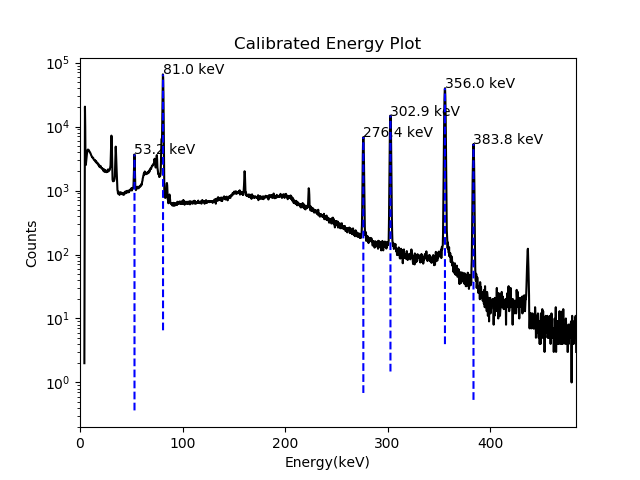
\includegraphics[width=0.5\linewidth]{images/Ba133_calibrated.png}
\caption{ ${133}$Ba spectrum with calibration fit}
\label{fig:BaSpec}
\end{figure}



\begin{table}[H]
        \begin{center}
                \begin{tabular}{ c c c c }
                        \textbf{Source} & \textbf{Energy (keV)} & \textbf{Calibration (keV)} & \textbf{abs(DeltaE) (keV)} \\
                        \hline
                        $^{133}$Ba      &      53.1622  &   53.087    & 0.074     \\5
                                                &       80.997  &       80.864  &       0.13    \\
                                                &       276.398 &       276.437 &       0.0272    \\
                                                &       302.853 &       302.805 &       0.0505   \\
                                                &       356.017 &       356.101 &       0.0968     \\
                                                &       383.851 &       383.871 &       0.0382    \\
                \end{tabular}
                \caption{Source Isotopes and Corresponding Gamma-ray energies}
                \label{tab:Comp}
        \end{center}
\end{table}
